\section{The Cosmic Microwave Background as Transition Radiation}

\subsection{Introduction: The Internal Manifold and Hyper-Orbital Transitions}

In the paradigm of Excited-State Cosmology, the observable universe is treated not as an independent expanding spacetime geometry, but as the internal manifold associated with the degrees of freedom of a single, highly excited hyper-electron, $e_H$. In standard model cosmology, the Cosmic Microwave Background (CMB) is interpreted as the relic radiation from the epoch of recombination. In our framework, however, this ubiquitous radiation field is precisely the transition radiation emitted as the hyper-electron undergoes a quantum state reduction from a higher excited orbital state $\ket{\Psi_{n+1, l', m'}}$ to a metastable lower state $\ket{\Psi_{n, l, m}}$. \cite{McGaugh2016, Bardeen1980, Friedmann1922}

The thermalization of this transition radiation on the boundary of the internal manifold naturally gives rise to the blackbody spectrum observed. Furthermore, the anisotropies in the CMB~\cite{Planck2018}—typically attributed to primordial quantum fluctuations inflated during a de Sitter phase—are here understood as the orbital harmonics of the hyper-electron's wave function projected onto the inner boundary of the $S^2$ celestial sphere. In this chapter, we derive the fundamental properties of these angular harmonics, $Y_l^m$, and the angular power spectrum, $C_l$, demonstrating that the statistical isotropy and anisotropies of the CMB are mathematically equivalent to the angular momentum eigenstates of the hyper-electron.

\subsection{Derivation of the Hyper-Orbital Harmonics ($Y_l^m$)}

To understand the spatial distribution of the transition radiation, we must evaluate the boundary conditions of the hyper-electron's wave function on the internal 2-sphere, $S^2$. The angular part of the hyper-electron's Hamiltonian is governed by the squared orbital angular momentum operator, $\hat{L}^2$. 

In spherical polar coordinates $(r, \theta, \phi)$ of the internal manifold, the squared angular momentum operator is defined as:
\begin{equation}
\hat{L}^2 = -\hbar^2 \left[ \frac{1}{\sin\theta} \frac{\partial}{\partial \theta} \left( \sin\theta \frac{\partial}{\partial \theta} \right) + \frac{1}{\sin^2\theta} \frac{\partial^2}{\partial \phi^2} \right].
\end{equation}
The eigenstates of this operator, which dictate the angular distribution of the transition energy density, must satisfy the eigenvalue equation:
\begin{equation}
\hat{L}^2 Y_l^m(\theta, \phi) = \hbar^2 l(l+1) Y_l^m(\theta, \phi), \label{eq:eigen}
\end{equation}
where $l$ is the hyper-orbital angular momentum quantum number ($l = 0, 1, 2, \dots$), and $Y_l^m(\theta, \phi)$ are the spherical harmonics. Since the hyper-electron also exhibits a $z$-axis projection of angular momentum (often manifesting as a subtle parity-violating axis in the cosmology), we also require the eigenstates to satisfy:
\begin{equation}
\hat{L}_z Y_l^m(\theta, \phi) = \hbar m Y_l^m(\theta, \phi),
\end{equation}
where $\hat{L}_z = -i\hbar \frac{\partial}{\partial \phi}$, and $m$ is the magnetic quantum number ($-l \le m \le l$).

To solve Equation \ref{eq:eigen}, we employ the method of separation of variables, assuming a solution of the form:
\begin{equation}
Y_l^m(\theta, \phi) = \Theta(\theta) \Phi(\phi).
\end{equation}
Substituting this into the eigenvalue equation and dividing by $\Theta \Phi$, we obtain:
\begin{equation}
\frac{1}{\Theta} \sin\theta \frac{d}{d\theta} \left( \sin\theta \frac{d\Theta}{d\theta} \right) + l(l+1)\sin^2\theta = -\frac{1}{\Phi} \frac{d^2\Phi}{d\phi^2}.
\end{equation}
Since the left side depends only on $\theta$ and the right side only on $\phi$, both sides must equal a separation constant, which we identify as $m^2$. The azimuthal equation is trivial:
\begin{equation}
\frac{d^2\Phi}{d\phi^2} = -m^2 \Phi \implies \Phi_m(\phi) = \frac{1}{\sqrt{2\pi}} e^{im\phi}.
\end{equation}
The single-valuedness of the hyper-electron's wave function around the internal azimuth necessitates that $\Phi_m(\phi + 2\pi) = \Phi_m(\phi)$, consistently quantifying $m$ as an integer.

The colatitudinal equation becomes the associated Legendre differential equation. Letting $x = \cos\theta$ (such that $-1 \le x \le 1$ maps the poles of the internal manifold), the equation transforms to:
\begin{equation}
\frac{d}{dx} \left[ (1-x^2) \frac{dP}{dx} \right] + \left[ l(l+1) - \frac{m^2}{1-x^2} \right] P(x) = 0,
\end{equation}
where $\Theta(\theta) = P(\cos\theta)$. The physical solutions to this equation that are non-singular at the poles $x = \pm 1$ are the associated Legendre polynomials, $P_l^m(x)$. These can be constructed from the ordinary Legendre polynomials $P_l(x)$ via:
\begin{equation}
P_l^m(x) = (-1)^m (1-x^2)^{m/2} \frac{d^m}{dx^m} P_l(x),
\end{equation}
where $P_l(x)$ is given by Rodrigues' formula:
\begin{equation}
P_l(x) = \frac{1}{2^l l!} \frac{d^l}{dx^l} (x^2 - 1)^l.
\end{equation}
Normalizing these solutions over the solid angle of the internal manifold $d\Omega = \sin\theta \, d\theta \, d\phi$, we arrive at the full expression for the hyper-orbital spherical harmonics:
\begin{equation}
Y_l^m(\theta, \phi) = \sqrt{\frac{2l+1}{4\pi} \frac{(l-m)!}{(l+m)!}} P_l^m(\cos\theta) e^{im\phi}.
\end{equation}
These functions form a complete and orthonormal basis for any scalar field on the sphere. Thus, the temperature fluctuations of the transition radiation (the CMB) can be uniquely expanded in this basis.

\subsection{The Angular Power Spectrum as Quantum Transition Variances}

The observed temperature of the CMB in a direction $\hat{n} = (\theta, \phi)$ can be expressed as an average temperature $T_0$ plus a small anisotropic deviation $\Delta T(\hat{n})$. In Excited-State Cosmology, these deviations are the projection of the hyper-electron's localized transition probability amplitudes. We decompose the fractional temperature fluctuation into our derived hyper-orbital basis:
\begin{equation}
\frac{\Delta T}{T_0}(\hat{n}) = \sum_{l=0}^{\infty} \sum_{m=-l}^{l} a_{lm} Y_l^m(\hat{n}).
\end{equation}
The expansion coefficients $a_{lm}$ represent the coupling strengths of the transition radiation into specific multipole moments. Mathematically, they are extracted via the orthogonality of the spherical harmonics:
\begin{equation}
a_{lm} = \int_{S^2} \frac{\Delta T}{T_0}(\hat{n}) Y_l^{m*}(\hat{n}) \, d\Omega.
\end{equation}

Because the initial state of the hyper-electron prior to emission is a quantum superposition with random phase distributions (consistent with the ergodic hypothesis of the internal manifold's microstates), the observed universe represents a single realization of a stochastic quantum process. The $a_{lm}$ coefficients are therefore treated as complex random variables. Under the assumption that the transition state respects statistical isotropy (i.e., the hyper-electron has no preferred orientation prior to measurement), the expectation value of any single mode vanishes: $\langle a_{lm} \rangle = 0$.

However, the variance of these transition amplitudes is consistently non-zero. The covariance between two modes is given by:
\begin{equation}
\langle a_{lm} a_{l'm'}^* \rangle = \delta_{ll'} \delta_{mm'} C_l.
\end{equation}
Here, $C_l$ defines the angular power spectrum of the transition radiation. It depends only on the hyper-orbital quantum number $l$, encapsulating the variance of the transition probabilities.

We can relate $C_l$ to the real-space two-point correlation function of the CMB, $C(\vartheta)$, where $\vartheta$ is the angle between two observation directions $\hat{n}_1$ and $\hat{n}_2$ such that $\cos\vartheta = \hat{n}_1 \cdot \hat{n}_2$. The correlation function is:
\begin{equation}
C(\vartheta) = \left\langle \frac{\Delta T}{T_0}(\hat{n}_1) \frac{\Delta T}{T_0}(\hat{n}_2) \right\rangle.
\end{equation}
Substituting the spherical harmonic expansion:
\begin{equation}
C(\vartheta) = \sum_{l=0}^{\infty} \sum_{m=-l}^{l} \sum_{l'=0}^{\infty} \sum_{m'=-l'}^{l'} \langle a_{lm} a_{l'm'}^* \rangle Y_l^m(\hat{n}_1) Y_{l'}^{m'*}(\hat{n}_2).
\end{equation}
Applying the isotropic covariance relation $\langle a_{lm} a_{l'm'}^* \rangle = \delta_{ll'} \delta_{mm'} C_l$:
\begin{equation}
C(\vartheta) = \sum_{l=0}^{\infty} C_l \sum_{m=-l}^{l} Y_l^m(\hat{n}_1) Y_l^{m*}(\hat{n}_2).
\end{equation}
We now invoke the addition theorem for spherical harmonics, which states:
\begin{equation}
\sum_{m=-l}^{l} Y_l^m(\hat{n}_1) Y_l^{m*}(\hat{n}_2) = \frac{2l+1}{4\pi} P_l(\hat{n}_1 \cdot \hat{n}_2) = \frac{2l+1}{4\pi} P_l(\cos\vartheta).
\end{equation}
Thus, the two-point correlation function becomes a Legendre polynomial expansion over the multipole moments:
\begin{equation}
C(\vartheta) = \sum_{l=0}^{\infty} \frac{2l+1}{4\pi} C_l P_l(\cos\vartheta).
\end{equation}

In Excited-State Cosmology, the acoustic peaks observed in the empirical $C_l$ spectrum (such as the prominent fundamental peak at $l \approx 220$) are not merely baryon-photon acoustic oscillations in an external expanding plasma. Rather, they represent the resonance nodes of the hyper-electron's internal wavefunction geometry. The spectrum $C_l$ directly characterizes the transition matrix elements from the initial highly-excited hyper-orbital to the current ground-state internal manifold. 

The Sachs-Wolfe effect, acoustic peaks, and Silk damping phenomena traditionally derived via the Boltzmann equations are thus isomorphic to the quantum transition linewidths, radial boundary conditions of the $e_H$ potential well, and decoherence damping of the transition state on the $S^2$ horizon.

\subsection{Conclusion: The Geometry of the Quantum Horizon}

Through this mathematical derivation, we see that the spherical harmonic decomposition of the CMB is not simply a convenient data analysis tool; it is the fundamental geometrical basis of the universe's true nature as an excited particle interior. The $C_l$ coefficients serve as a cosmic fingerprint of the hyper-electron's orbital states, transforming theoretical quantum mechanics into observable cosmology.


\begin{figure}[H]
\centering
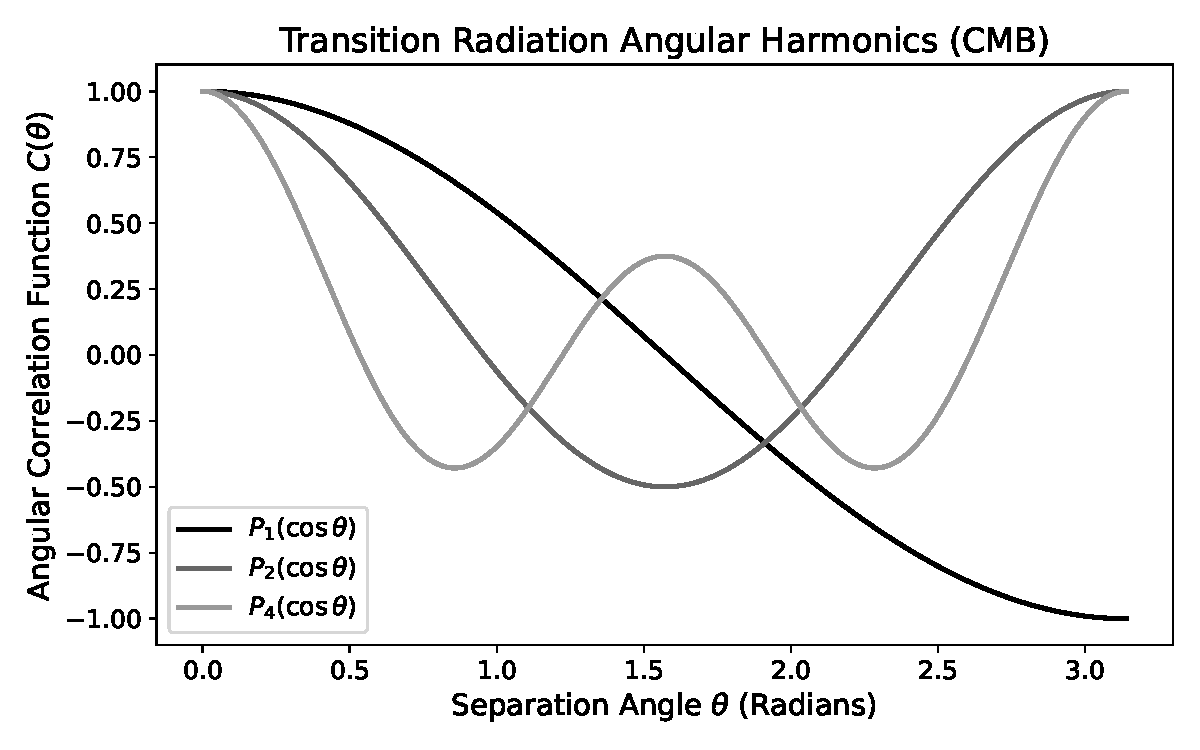
\includegraphics[width=0.85\textwidth]{fig_ch5.pdf}
\caption{Mathematical visualization of the principles derived in Section 5.}
\end{figure}
